
	A robot autonomy level can be measured by the percentage of time that a robot does not need intervention to realize a task \cite{hri:Yanco04classifyinghuman-robot}. Nowadays robots are still not completely prepared to be autonomous and understand our language, but they have become useful in many tasks as helpers \cite{hri:robonaut}. \ac{HRI} is responsible for the way of ``communicating'' with a robot and control how it may help us in a task.

	The humanoid control problem as been approached by several works in the past and used multiple different solutions. One of those solutions has been telepresence \cite{hri:1512452} that allows the remote control of a robot. The novel devices that are used in this dissertation allow for that type of remote control. Using these devices it is possible to do motion capture of the users movements and map it to the robot to enable learning by demonstration techniques, as shown in other works \cite{hri:5480475}.
	
	In the last few years there were several gaming interfaces introduced by gaming companies that have contributed for the development of the \ac{HCI}, and from which \ac{HRI} has taken advantage. These interfaces have been compared with each other by other works \cite{hri:eu}, and considered as suitable for motion capture. With these controllers it is possible to build cheap and robust motion capture systems for \ac{HRI}.

	The iCub is a 140cm tall humanoid robot child, that is able to crawl, sit, and do sophisticated manipulation with its hands. The iCub has 53 \ac{DOF}, 39 \ac{DOF} that are distributed through the upper part of the robot body, and 14 \ac{DOF} are in the lower part. The iCub project is all open source, which makes all the development of the iCub available to anyone interested. This software can be all downloaded form the iCub website\footnote{\url{http://www.robotcub.org/}} \cite{icub:Metta:2008:IHR:1774674.1774683}. Each joint of the iCub as at least one motor that can be controlled through a server framework called \ac{Yarp}. All the low level control is made through a set of \ac{DSP} based cards, connected via \ac{CAN} bus, specifically designed for the iCub robot\cite{icub:icub2010NN}. The sensor and motor-state data is passed on to the PC104 card located in the head of the robot, where all that data is reformatted and synchronized with data streams to a Gbit Ethernet connection. Typically the heavier computation is made on independent machines external to the iCub, connected through the iCub Ethernet connection.
	
	An \ac{Yarp} network provides access and control to the iCub motor joints. The main abstractions of \ac{Yarp} are the \verb\ports\. \verb\Ports\ implement the observer pattern that allows to send a message through one port, to a multiple number of ports that are distributed across different computers, this way the sender and receiver can work independently. Another abstraction implemented by \ac{Yarp} is the \verb\device\, that allows to specify which device the programmer/user wants to interact with and the framework provides an object that hides the low-level programming details. This pair of \verb\port\/\verb\device\ allows for the development of a remote device driver that can be used across a network, making the heavier processing independent from the robot hardware.

 	\begin{figure}[htb]
	\begin{center}
	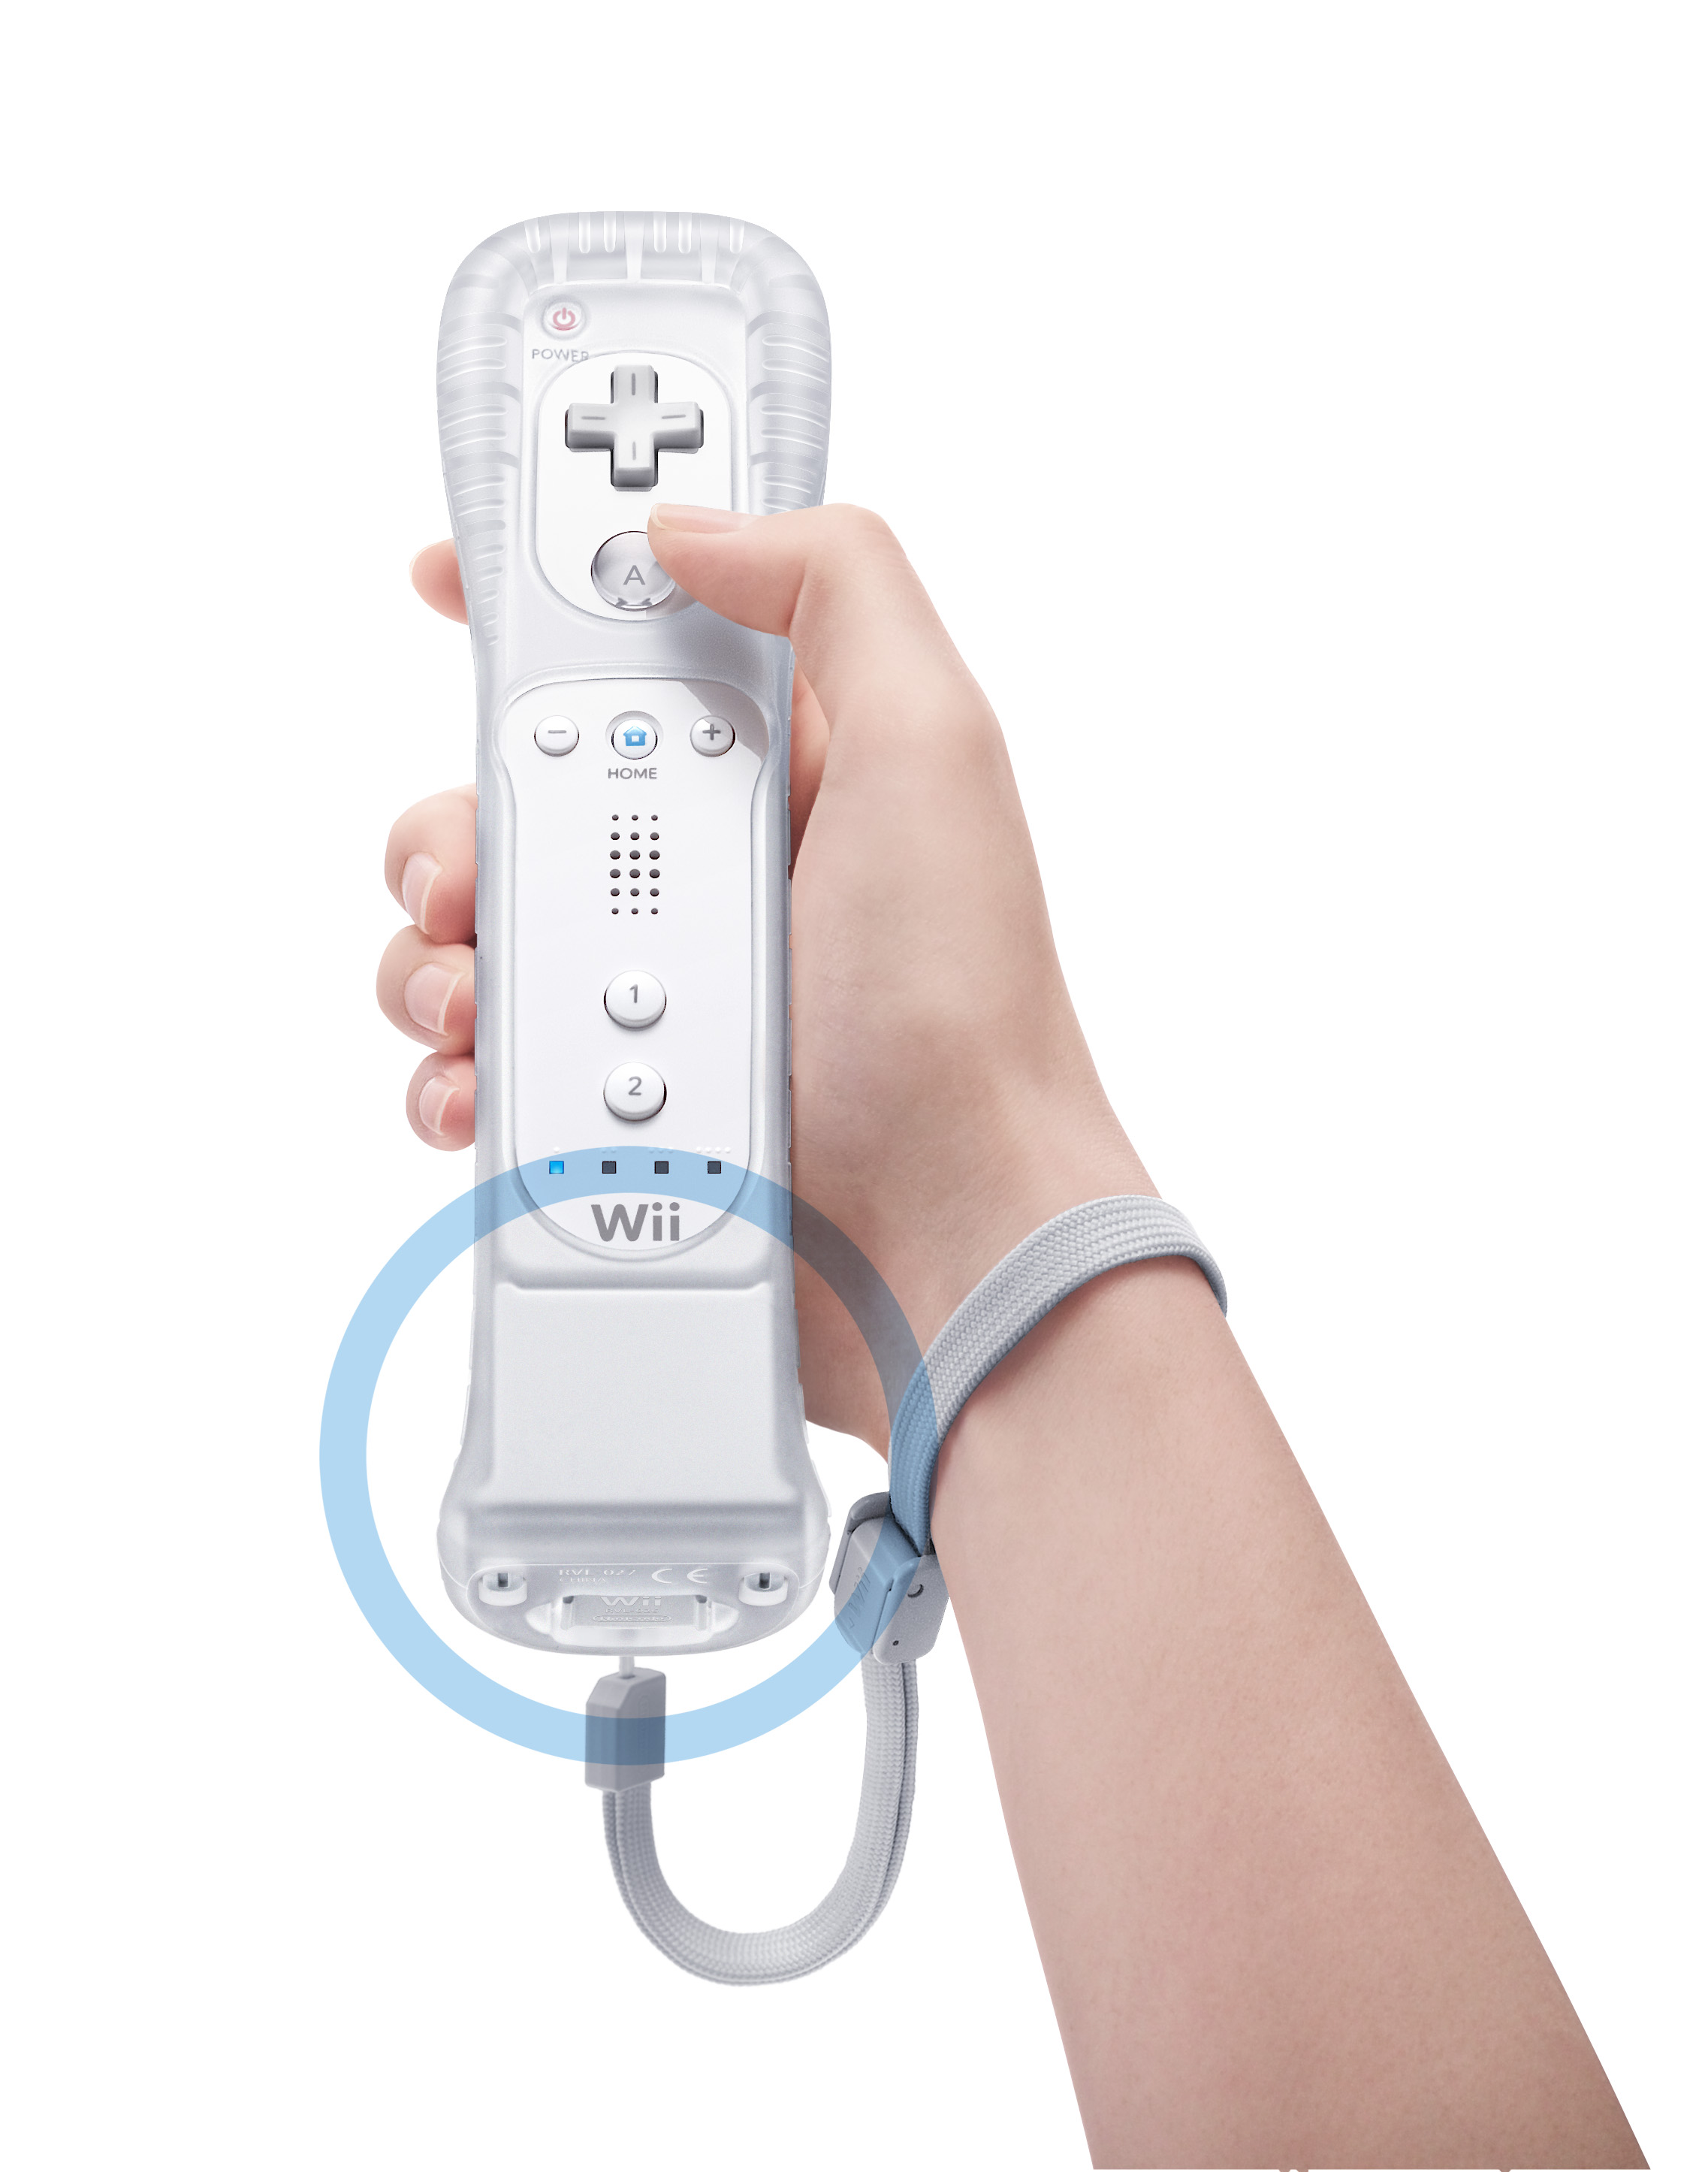
\includegraphics[height=70mm]{wiimotemotionplus.jpg}
	\end{center}
	\caption[Wiimote with the Motion Plus extension attached]{Wiimote with the Motion Plus extension attached.} 
	\label{fig:wiimotemotionplus}
	\end{figure}

	The \ac{Wiimote} (figure \ref{fig:wiimotemotionplus}) is the novel remote control used with the Wii gaming console. Its many attractions are that it provides unique interaction possibilities, it is inexpensive \cite{springerlink:robotontheleash,wiimote:azmi2009wiimote} and durable. What allows for unique interaction possibilities is the accelerometer that can get the current orientation of the remote, and the amount of force applied to the remote in respect to the gravity \cite{wiimote:Guo:2008:EUT:1357054.1357076}. This categorizes this device as a spatial convenient device \cite{wiimote:10.1109/MCG.2009.109}, making it respect the three main spatial characteristics: provides spatial data, has sensors and emitters, also it is robust, cheap, and easily configured. Also the \ac{Wiimote} has an extension port, through which it is possible to extend the \ac{Wiimote} capabilities. The extension used for the work developed was the \ac{MP} extension, that enables a better motion capture by adding a gyroscope to the \ac{Wiimote} features. Inside the \ac{MP} there is a dual-axis gyro by InvenSense, the IDG-600(pitch and roll), and a single-axis gyro by EPSON TOYOCOM labeled X3500W (yaw). These two gyroscopes allow to measure the rate of rotation along all 3-axes of X (pitch), Y (roll), and Z (yaw).
	
	The works that use this device range from motion control systems \cite{wiimote:lowcostmultipledegrees}, to robotic user interface \cite{wiimote:bascetincelik2009wiirobot}, or even art projects \cite{WiiArts:Lee:2008:WCC:1347390.1347400}. The flexibility and ease of use has been presented as a efficient interface for robotic control on several works \cite{springerlink:robotontheleash,wiimote:bascetincelik2009wiirobot,wiimote:Guo:2008:EUT:1357054.1357076}. These works typically compare traditional interface methods with the \ac{Wiimote} interface, where the accelerometer and \ac{IR} camera are used to control a robot or a 3D environment.

 	\begin{figure}[htb]
	\begin{center}
	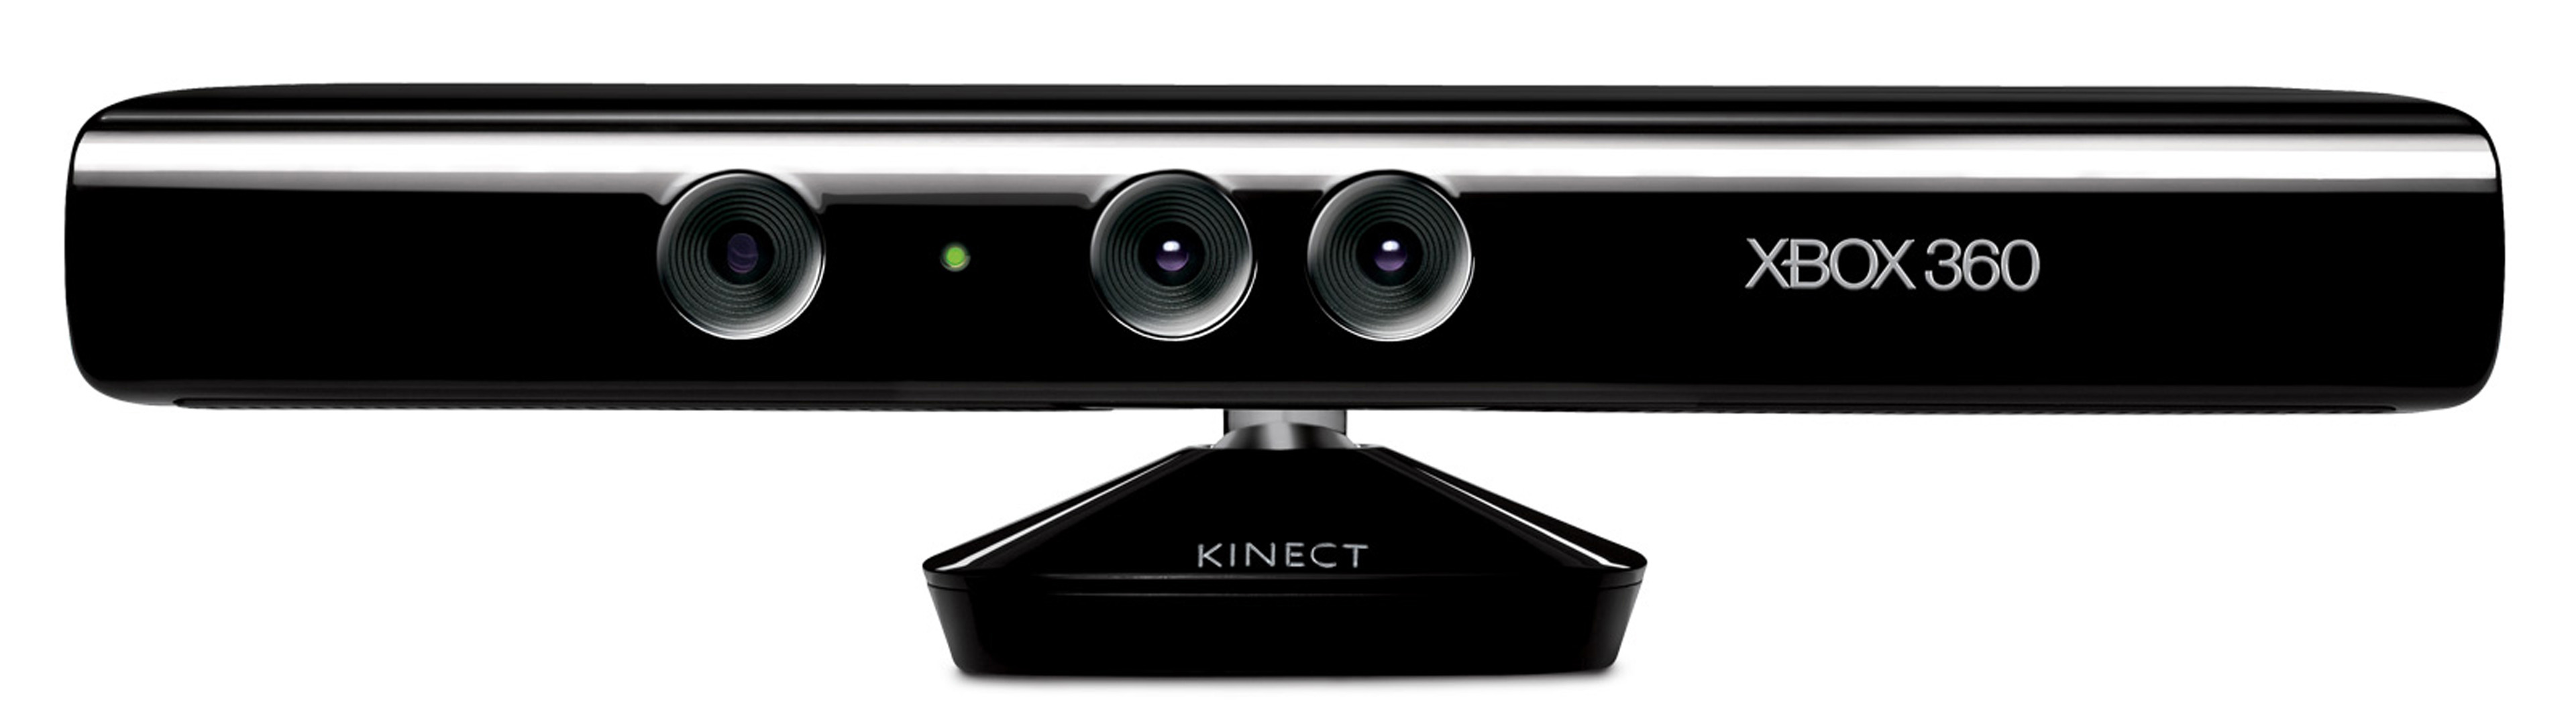
\includegraphics[width=70mm]{kinectsensor.jpg}
	\end{center}
	\caption[Microsoft Kinect sensor]{Microsoft Kinect sensor.} 
	\label{fig:kinectsensor}
	\end{figure}

	The Kinect for the Xbox 360 console from Microsoft\footnote{\url{http://www.xbox.com/en-US/Kinect/}}, is a webcam style device add-on that allows a controller free gaming interaction.	The technology used by the Kinect to produce its result is quite old, but the algorithms that it uses for skeleton detection and user tracking are the ones being presented as innovations in the gaming world. The systems that are used with this sensor allow to control games using the user body without any type of controller in the user hands. As Microsoft puts it ``you are the controller''\footnote{\url{http://www.microsoft.com/presspass/features/2010/oct10-/10-21kinectads.mspx}}. Due to its low price and since there are a few free \acp{API} being released, there has been an exponential rise in the amount of projects done using the Kinect. From NASA\footnote{\url{http://www.sfgate.com/cgi-bin/article.cgi?f=/c/a/2011/01/10/BUO01H4ISI.DTL}} to researchers and hobbyists, have contributed to a very steep and interesting evolution in the natural interfaces community using this device. Those projects show many times original, and unexpected uses of the Kinect for different projects.

	\begin{figure}[htb]
	\begin{center}
	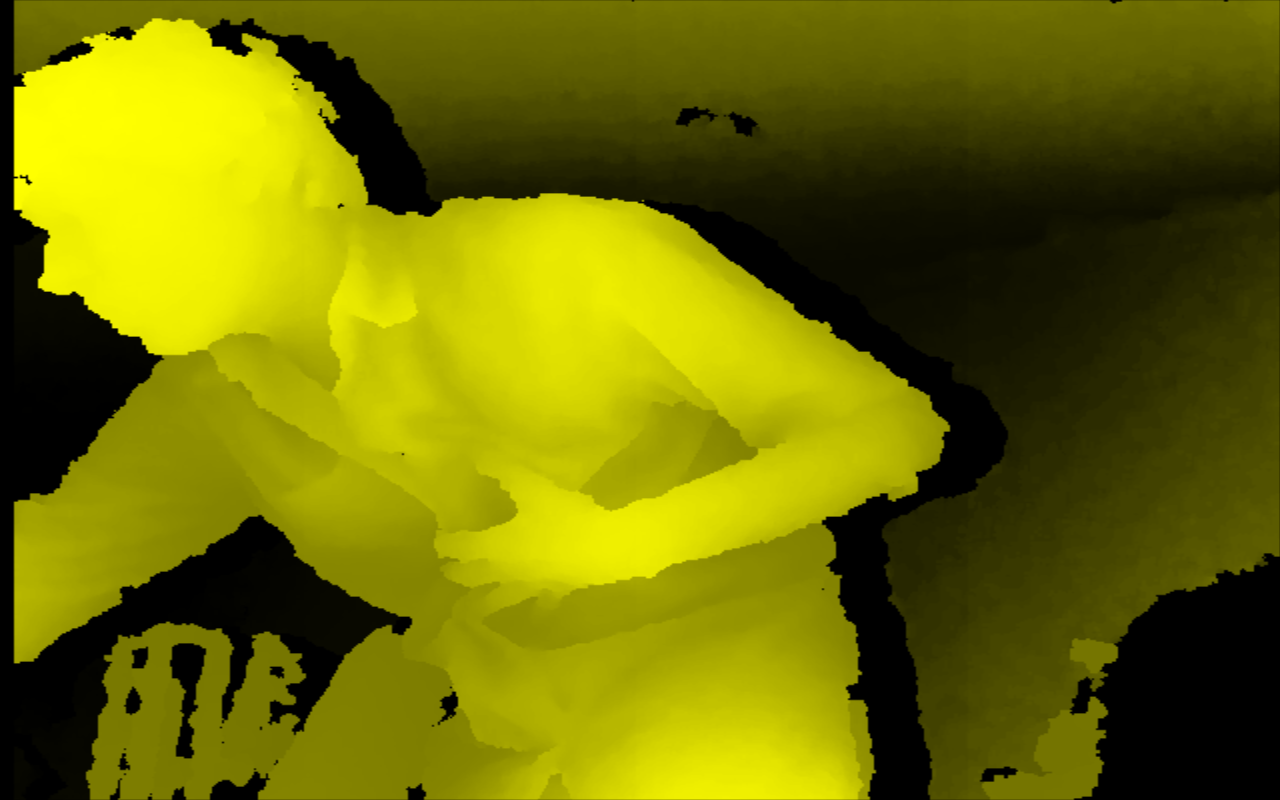
\includegraphics[width=70mm]{KinectDepthImage.png}
	\end{center}
	\caption[Kinect depth image]{Kinect sensor depth image example.} 
	\label{fig:kinectDepthImage}
	\end{figure}
	
	The Kinect can capture a depth-image where each pixel indicates also its depth. To achieve such an image several different techniques can be used, the most typical are: stereo imaging, \ac{TOF} cameras, and structured light. The Kinect uses a structured light pattern that is projected by the \ac{IR} light source. The image of that projection is captured by an \ac{IR} camera in the Kinect. The deformations in that light pattern are interpreted by the Kinect software to detect what is the distance of each pixel captured. Recently Microsoft acquired a company that produces \ac{TOF} cameras and it is rumored that the next version of Kinect might use \ac{TOF} instead of the structured light technique\footnote{\url{http://www.nytimes.com/2010/10/30/technology/30chip.html}}. This preference is due to the quality of the depth image calculated, that is higher in a \ac{TOF} camera, and also more robust to different environments.